\newpage
\chapter{Einführung}
\section{Installation}
Das folgende Setup wird vorausgesetzt:
\begin{itemize}
    \item Windows 10
    \item \gls{IDE} Visual Studio Community 2019 oder höher mit C++ \footnote{\url{https://visualstudio.microsoft.com/de/downloads/}}
    \item \gls{CMake} in der Version 3.18.2 \footnote{\url{https://cmake.org/download/}}
    \item \gls{Python} in der Version 3 \footnote{\url{https://www.python.org/downloads/windows/}} (Füge Python der Pfad-Variable hinzu)
\end{itemize}
Als Alternative kann auch CLion \footnote{\url{https://www.jetbrains.com/de-de/clion/download/}} als IDE verwendet werden.
Diese ist jedoch nicht frei erhältlich. Achtung, da auch CLion den MSVC++ verwendet, muss Visual Studio Community 2019
ebenfalls installiert werden.

\subsection{MS Visual Studio 2019 konfigurieren}
Sobald sichergestellt ist, dass obig aufgeführte Voraussetzungen gegeben sind, kann die IDE MS Visual Studio 2019
gestartet werden. Führe die folgenden Schritte durch:
\begin{itemize}
    \item Auf der rechten Seite siehst du diverse Optionen, um ein Projekt zu öffnen oder zu erstellen. Wähle dort
    'Lokalen Ordner öffnen' aus.
    \item Navigiere zu deinem Verzeichnis, in das du das Projekt gespeichert hast.
    \item Öffne den Projektornder (meistens 'learn\textunderscore with\textunderscore tello').
    \item Nun wird das Projekt geöffnet und die CMake-Generierung gestartet, welche eventuell fehlschlagen wird.
    Sollte dies der Fall sein, so ist die CMake-Version des Visual-Studios zu gering und wir müssen diese manuell
    einstellen. Öffne in dem Fall den Explorer und navigiere in deinen Projektordner. Dort siehst du die Datei 'CMakeSettings.json'.
    Öffne diese in einem Editor und füge die folgende Zeile hinzu:\\
    \begin{lstlisting}[language=json, basicstyle=\small]
    {
        ...
        "cmakeExecutable": "D:\\Prog\\CMake-3.18.2\\bin\\cmake.exe"
        ...
    }
    \end{lstlisting}
    \item Sobald diese Änderungen gemacht sind und du zurück ins Visual Studio wechselst, siehst du, dass CMake bereits
    die Generierung gestartet hat. CMake macht nun in einem ersten Schritt das Basissetup, um der IDE mitzuteilen,
    wie das Projekt aufgebaut und wie die 'targets' generiert werden sollen.
\end{itemize}
Sobald CMake fertig ist, kannst du nun die nachfolgend aufgeführten 'Startelemente' erstellen.
Um dies zu bewerkstelligen, verschaffst du dir zuerst einen kleinen Überblick der IDE. Im Zentrum steht das
Code-Fenster, welches den meisten Platz einnimmt. Auf der rechten Seite siehst du den Projektmappen-Explorer. Dort
werden die verschiedenen Verzeichnisse sowie der Code gelistet.
Oben kannst du einen grünen Play-Button sehen, daneben steht zu Beginn 'Startelement auswählen'. Klappe dieses auf
und du solltest mindestens folgende Startelemente sehen:
\begin{description}
    \item[00\textunderscore base\textunderscore module.dll] Beinhaltet Basiseinstellungen für die Drohne(n)
    \item[01\textunderscore keyboard\textunderscore module.dll] Die ersten paar Übungen.
    \item[01\textunderscore keyboard\textunderscore module\textunderscore solution.dll] Die Lösungen zu den Übungen.
    \item[99\textunderscore template.dll] Dies ist eine Vorlage für neue Module, das kann ignoriert werden.
    \item[app\textunderscore basic.exe] Die Hauptapplikation (Um diese zu starten, drücke den grünen Play-Button hinter dem Dropdown mit den 'targets')
    \item[app\textunderscore common\textunderscore video.dll] Eine Bibliothek mit Code, den Module verwenden können.
\end{description}
Um ein Startelement zu kompilieren, muss dieses ausgewählt werden. Danach drückst du den Play-Button, um den Build
zu starten.\\
Für den Anfang reicht es, wenn die folgenden Startelemente erstellt werden (Achtung, nach dem Build einer .dll wird ein
Fehler angezeigt, dass diese nicht ausgeführt werden kann. Das ist ganz normal, klicke den Fehler einfach weg und
schliesse die automatisch geöffnete Datei launch.vs.json ohne zu speichern):
\begin{itemize}
    \item 00\textunderscore base\textunderscore module.dll
    \item 01\textunderscore keyboard\textunderscore module.dll
    \item app\textunderscore common\textunderscore video.dll
    \item app\textunderscore basic.exe
\end{itemize}
Schliesse die nun geöffnete Anwendung.\\
Wenn die Builds allesamt ohne Fehler durchlaufen, dann kannst du deine Tello-EDU-Drohne starten.
Du solltest sie zuerst mit der offiziellen App kalibrieren.
Stelle sie danach auf den Boden, wo genug Platz drumherum und nach oben ist. Die Drohne sollte gelb blinken, das heisst,
sie wartet auf eine Verbindung. Wähle in den WLAN-Einstellungen das Tello-EDU WLAN aus.\\
Wähle nun das Startelement 'app\textunderscore basic' aus und drücke den Play-Button. Um deine Umgebung zu testen, drücke
den Button 'Take off' in der Applikation. Wenn die Drohne fliegt und du das Kamerabild der Drohne siehst, hast du alles richtig gemacht
und kannst nun mit den Übungen starten. Drücke den Knopf nochmals, um die Drohne zu landen und schliesse die Applikation.
\newpage
\subsection{CLion konfigurieren}
Wenn CLion als IDE verwendet wird, so müssen die folgenden Schritte durchgeführt werden.
In einem ersten Schritt wird CLion geöffnet und über 'File - New Project' ein neues Projekt ersetllt.
Nun muss das höchste CMakeLists.txt file des Repositorys 'learn\textunderscore with\textunderscore tello' ausgewählt werden.
Danach kann die Build-Umgebung eingerichtet werden.

\begin{itemize}
    \item Öffne 'File - Settings'
    \item Navigiere zu 'Build, Execution, Deployment'
    \item Wähle 'Toolchains' aus
    \item Prüfe, ob eine Toolchain namens 'Visual Studio' verfügbar ist.
    Wenn ja, erübrigen sich die weiteren Schritte.
    \item Drücke den 'Add'-Button in der oberen linken Ecke
    \item Nun muss die Umgebung ausgewählt werden. Beachte das nachfolgende Bild.
    Es muss mindestens eine CMake-Version 3.18.2 verfügbar sein.\par
    \begin{minipage}{\linewidth}
        \centering
        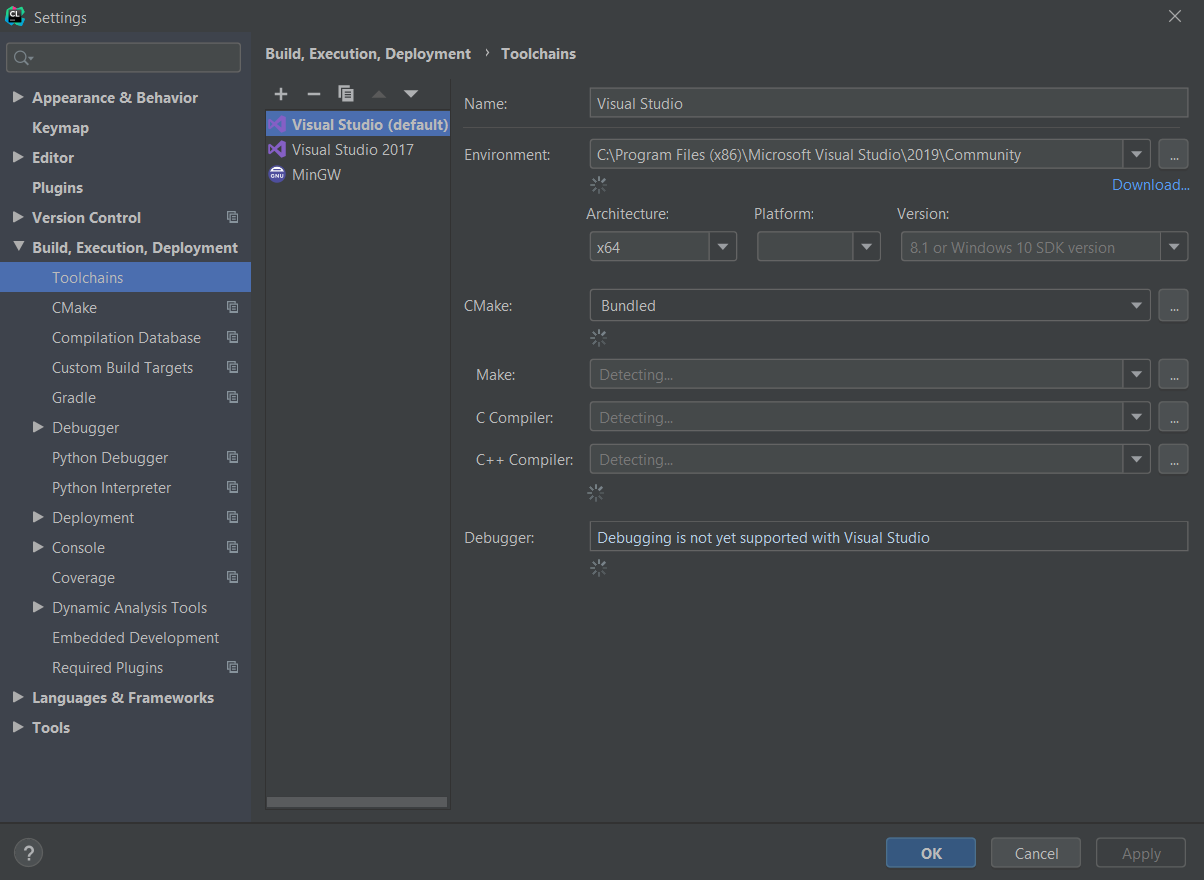
\includegraphics[width=0.6\textwidth]{../common/chapter_01/resources/01_clion_configure_toolchain.png}
        \captionof{figure}{CLion toolchain Konfiguration}
    \end{minipage}
\end{itemize}
Nun bist du in der Lage, das Projekt im 'Debug'-Modus zu erstellen. Damit ist gemeint, dass zu jeder Library oder jeder
ausführbaren-Datei (executable) zusätzlicher Code der Applikation hinzugefügt wird. Dadurch wird das Binary ungefähr zehn mal langsamer.
Wenn du die Applikation im Release-Modus erstellen willst, dann musst du die folgenden Schritte durchführen.
Im Release-Modus kann eine Applikation nicht mehr schrittweise durchlaufen werden, dafür ist sie viel performanter.
Dieser Modus wird verwendet, wenn eine Applikation fertig ist und sich nicht mehr in der Entwicklungsphase befindet.
\begin{itemize}
    \item Öffne 'File - Settings'
    \item Navigiere nach 'Build, Execution, Deployment'
    \item Wähle 'CMake' aus
    \item Prüfe, ob ein Profil namens 'Release' verfügbar ist. Wenn ja, dann ist bereits alles eingerichtet.
    \item Drücke den 'Add'-Button in der oberen linken Ecke.
    \item Ein neuer Eintrag wird erstellt. Benenne ihn 'Release', wenn dies nicht schon der Fall ist.
\end{itemize}
Nun werden die CMake-Konfigurationen neu erstellt. Nach diesem Vorgang, kannst du einen Blick in die obere rechte Ecke
von CLion werfen. Dort siehst du ein grünes Hammersymbol. Daneben befindet sich ein Dropdown, wo die verschiedenen
'targets' (Ziele) ausgewählt werden können. Die Konfiguration wird dahinter ausgegeben. Dies ist entweder 'Debug' oder
'Release'. Wenn du das Dropdown ausklappst, kannst du sehen, dass du zwischen diesen Konfigurationen 'Debug' und 'Release'
sowie allen 'targets' wechseln kannst. Ein 'target' wird in diesem Kontext als library oder executable-file verstanden.
Es kann aber auch etwas spezielleres sein wie zum Beispiel ein Vorgang, um Dateien von einem Verzeichnis in ein anderes
zu kopieren.\\
Die folgenden 'targets' sollten vorhanden sein (Es werden nicht alle aufgeführt):
\begin{description}
    \item[00\textunderscore base\textunderscore module] Beinhaltet Basiseinstellungen für die Drohne(n)
    \item[01\textunderscore keyboard\textunderscore module] Die ersten paar Übungen.
    \item[01\textunderscore keyboard\textunderscore module\textunderscore solution] Die Lösungen zu den Übungen.
    \item[99\textunderscore template] Dies ist eine Vorlage für neue Module, das kann ignoriert werden.
    \item[app\textunderscore basic] Die Hauptapplikation (Um diese zu starten, drücke den grünen Play-Button hinter dem Dropdown mit den 'targets')
    \item[app\textunderscore common] Eine Bibliothek mit Code, den alle Module verwenden.
    \item[app\textunderscore common\textunderscore video] Eine Bibliothek mit Code, den Module verwenden können.
\end{description}
Um ein 'target' zu kompilieren, muss dieses im Dropdown ausgewählt werden. Danach wird der grüne Hammer daneben
geklickt. Für den Anfang reicht es, wenn die folgenden 'targets' erstellt werden:
\begin{itemize}
    \item app\textunderscore basic
    \item 00\textunderscore base\textunderscore module
    \item 01\textunderscore keyboard\textunderscore module
\end{itemize}
Wenn die Builds allesamt ohne Fehler durchlaufen, dann kannst du deine Tello-EDU-Drohne starten.
Du solltest sie zuerst mit der offiziellen App kalibrieren.
Stelle sie danach auf den Boden, wo genug Platz drumherum und nach oben ist. Die Drohne sollte gelb blinken, das heisst,
sie wartet auf eine Verbindung. Wähle in den WLAN-Einstellungen das Tello-EDU WLAN aus.\\
Wähle nun das 'target' 'app\textunderscore basic' aus und drücke den Play-Button. Um deine Umgebung zu testen, drücke
den Button 'Take off' in der Applikation. Wenn die Drohne fliegt und du ein Bild siehst, hast du alles richtig gemacht
und kannst nun mit den Übungen starten. Drücke den Knopf nochmals, um die Drohne zu landen und schliesse die Applikation.
\newpage
\section{Architektur}
Das Projekt besteht aus einer ausführbaren Applikation (app\textunderscore basic), welche grundsätzlich nur alle \glspl{Plugin} lädt.
Die Plugins bilden die eigentlich wichtigen Teile der Applikation, sie beinhalten die Übungen und Lösungen.
Jedes Plugin ist eine in sich abgeschlossene Anwendung, welche für einen spezifischen Use-Case erstellt wurde, z.B.
das Fliegen der Drohne mithilfe der Tastatur oder das Fliegen der Drohne über Objekterkennung.
\begin{figure}[H]
    \centering
    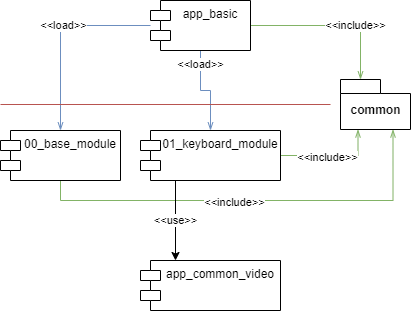
\includegraphics[width=0.6\textwidth]{../common/chapter_01/resources/02_architecture.png}
    \captionof{figure}{Architektur}
\end{figure}
Wenn du in einem der Module (Plugin) Änderungen gemacht hast, dann musst du dieses Modul neu kompilieren. Wähle
dazu dieses Modul als Startlement in Visual Studio 2019 oder als 'target' in CLion aus und führe die Kompilierung
durch. Wenn du anschliessend die Hauptapplikation startest, wirst du deine Änderungen sehen.
Wenn du bei einer Aufgabe nicht weiter wissen solltest, kannst du einen Blick in die Referenzimplementation werfen.
Diese enden mit der Bezeichnung '\textunderscore solution'. Jeder Übungsabschnitt beinhaltet die entsprechenden
Lösungen am Ende des Kapitels.
Und nun, viel Spass bei den Übungen.